\documentclass[aspectratio=169]{beamer}

\usepackage[utf8]{inputenc}
\usepackage[english]{babel}
\usepackage{multicol}
\usepackage{tabulary}
\usepackage{hyperref}
\usepackage{tikz}
\usepackage{mathtools}

\let\oldsection\section
\renewcommand{\section}[1]{
    \oldsection{#1}	
    \subsection{}
}

\setbeamerfont{section in toc}{size=\LARGE}

\newenvironment{myframe}[1][t]{\begin{frame}[#1]{\secname}{\subsecname}}{\end{frame}}

\usetheme{cranfielduniversity}

\usepackage[sorting=none, backend=biber, style=numeric, doi=false, isbn=false, url=false, eprint=false, date=year, hyperref]{biblatex}

\addbibresource{../library.bib}
\addbibresource{../my_references.bib}

\author{Baptiste NOGARET}
\title{Automated food log}

\supervisor{Dr Stefan RÜGER}

\setcounter{tocdepth}{1}

\begin{document}
	
	\begin{frame}[plain]
		\titlepage
	\end{frame}
    
    \begin{frame}{Table of contents}
        {
            \renewcommand{\baselinestretch}{1.5}\normalsize
            \begin{multicols}{2}
                \tableofcontents
            \end{multicols}
        }
    \end{frame}
    
    \section{Why a food log analysis system?}
    
    {
        % Disable footline for this frame
        \setbeamertemplate{footline}{}
    	\begin{myframe}
            \begin{figure}[h]
                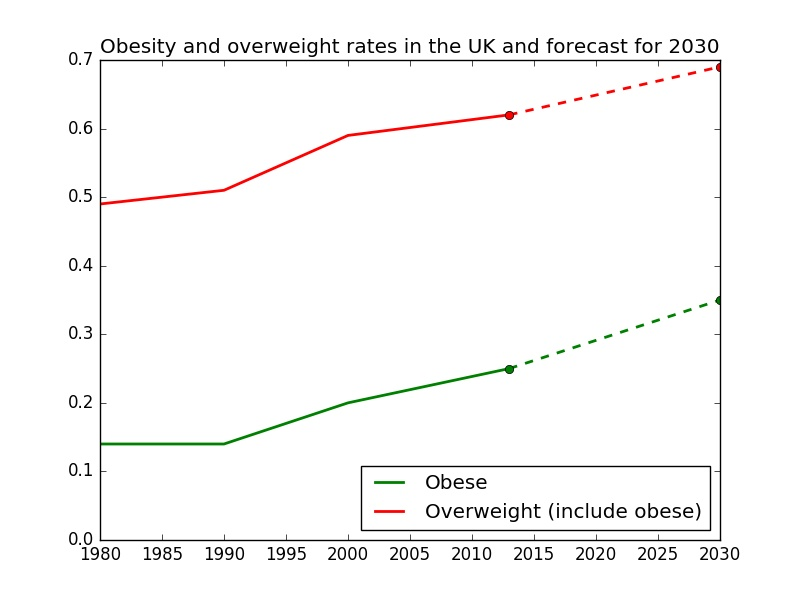
\includegraphics[width=0.5\textwidth,  height=0.45\textwidth ]{../img/obesity_uk}
                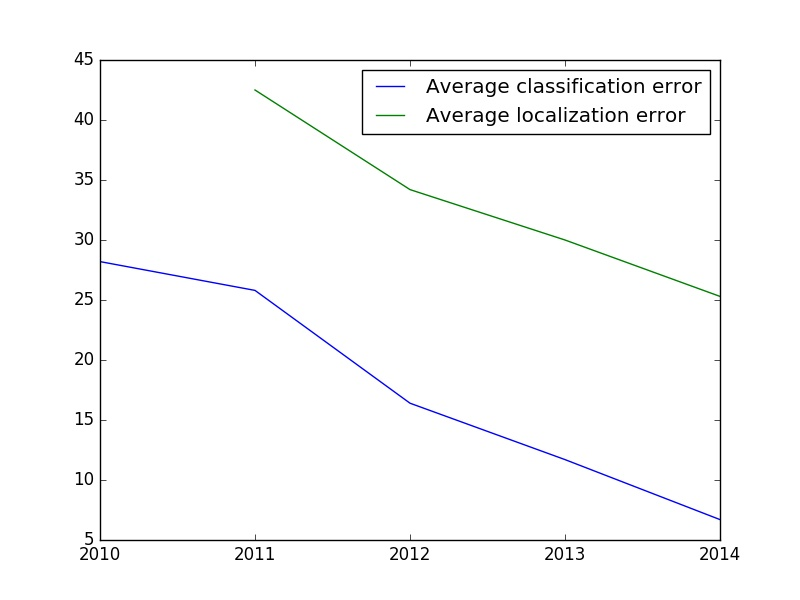
\includegraphics[width=0.5\textwidth,  height=0.455\textwidth ]{../img/imagenet}
            \end{figure}
    	\end{myframe}
    }
    
     \section{Overall process}
     
     \begin{myframe}
         Roughly copying the procedure of FoodLog \cite{Kitamura2009, Kitamura2008, DeSilva2011, Aizawa2013, Kagaya2014}:
         \begin{itemize}
             \item Generate a relevant dataset
             \item Extract characteristic
             \item Learn
             \item For a new picture from a user, classify and estimate intake
         \end{itemize}
         Focus on the first three points
     \end{myframe}
    
    \section{Challenges}
    {
        \author{}
        \begin{myframe}
            \begin{columns}
                \column{0.5\textwidth}
                \centering
                High intra-class variability
                \begin{figure}[h]
                    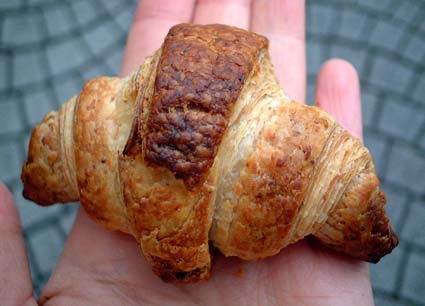
\includegraphics[width=0.7\textwidth, height=0.4\textwidth]{../img/croissant_2}
                    \vfill
                    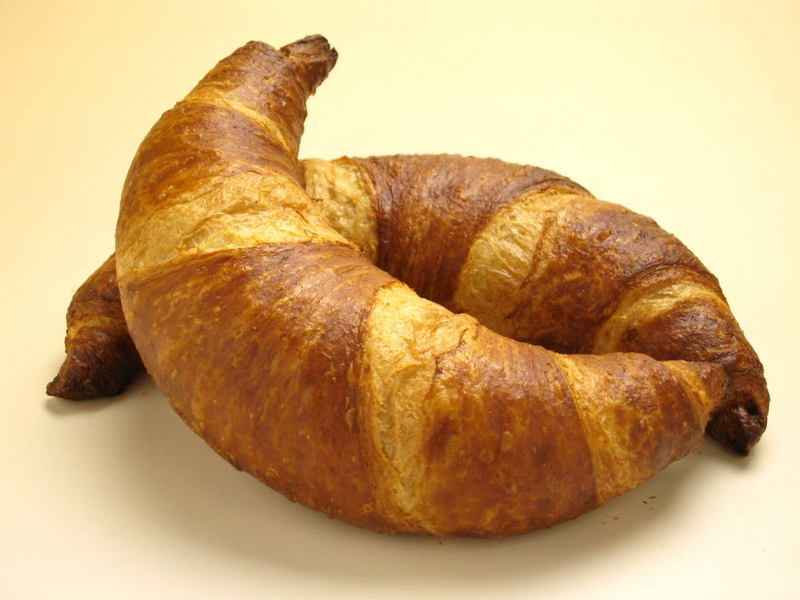
\includegraphics[width=0.7\textwidth, height=0.4\textwidth]{../img/croissant_3}
                \end{figure}
                
                \column{0.5\textwidth}
                \centering
                Low inter-class variability
                
                \begin{figure}[h]
                    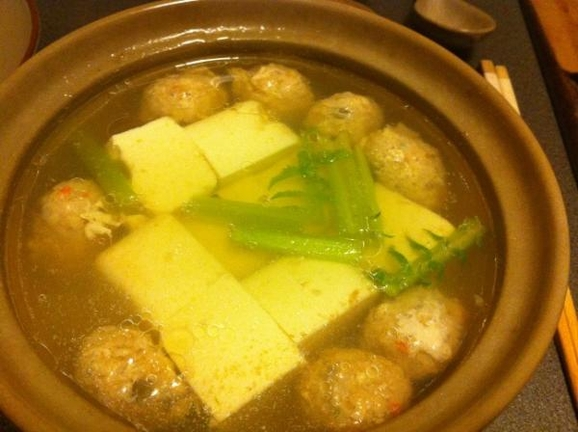
\includegraphics[width=0.7\textwidth, height=0.4\textwidth]{../img/clear_soup}
                    \vfill
                    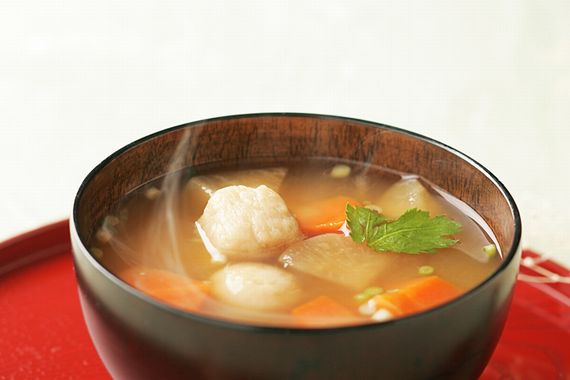
\includegraphics[width=0.7\textwidth, height=0.4\textwidth]{../img/miso_soup}
                \end{figure}
            \end{columns}
        \end{myframe}
    }

    \section{Dataset}
    
     \begin{myframe}
         \begin{center}
             %\setlength{\tabcolsep}{5pt} % Default value: 6pt
             \renewcommand{\arraystretch}{1.3} % Default value: 1
             \begin{tabulary}{\textwidth}{|| c | C C C C C||}
                 \hline
                 Name & Release date & Number of pictures & Type of food & Number of classes & Multiple food items \\
                 \hline\hline
                 PFID \cite{Chen2009} & 2009 & 4545 & American fast-food  & 101 & No \\
                 \hline
                 UEC FOOD 100 \cite{Matsuda2012a} & 2012 & 14361 & Japanese & 100  & Yes \\
                 \hline
                 FIDS 30 \cite{FIDS30} & 2013 & 971 & Fruit & 30 & No \\
                 \hline
                 ETHZ Food-101 \cite{Bossard2014} & 2014 & 101 000 & European & 100 & No \\
                 \hline
                 FooDD \cite{ParisaPouladzadehAbdulsalamYassine2015} & 2015 & 3000 & Fruit & 23 & Yes \\
                 \hline
                 \textbf{UEC FOOD 256} \cite{Kawano2015} & \textbf{2015} & \textbf{31395} & \textbf{World} & \textbf{256}  & \textbf{Yes} \\ 
                 \hline
             \end{tabulary}
        \end{center}
    \end{myframe}
    
    {
        \author{}
        \subsection{Example of multi-items}
        
        \begin{myframe}
            \begin{figure}[h]
                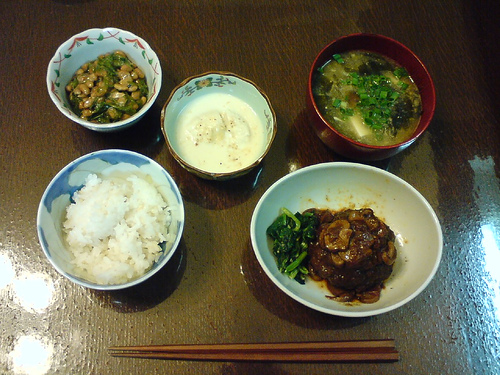
\includegraphics[width=0.4\textwidth,  height=0.4\textwidth ]{../img/multiple_food_items_1}
                \vspace{2cm}
                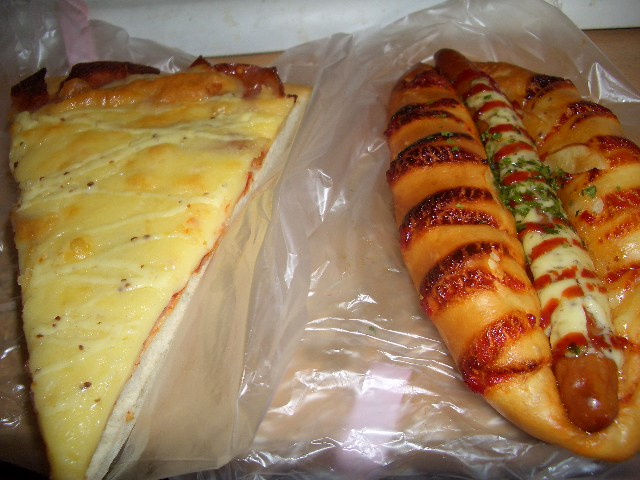
\includegraphics[width=0.4\textwidth,  height=0.4\textwidth ]{../img/multiple_food_items_4}
            \end{figure}
        \end{myframe}
    }
    
    \section{Feature description}
    
    \subsection{Bag of visual words}
    
    \begin{myframe}
        Overall process:
        \begin{enumerate}
            \item Keypoints detection (dense grid / SIFT \footfullcite{Lowe2004} / SURF)
            \item Keypoints description (SIFT or SURF)
            \item Clustering to get N words (k-means clustering)
            \item Express each picture by an histogram of visual words
        \end{enumerate}
    \end{myframe}
    
    \subsection{Local binary pattern}
    
    \begin{myframe}
        Use in \cite{Zong2010, Nguyen2014} for texture classification
        
        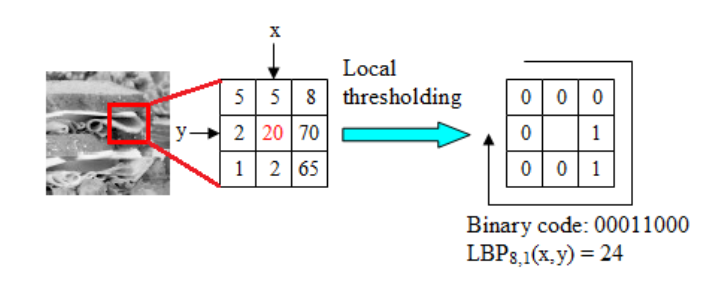
\includegraphics[scale=0.55]{../img/lbp}
    \end{myframe}
    
    \subsection{Color moments and histograms}
    
    \begin{myframe}
        \begin{columns}
            \column{0.7\textwidth}
            \centering
            % Joint histogram:
            \begin{figure}[h]
                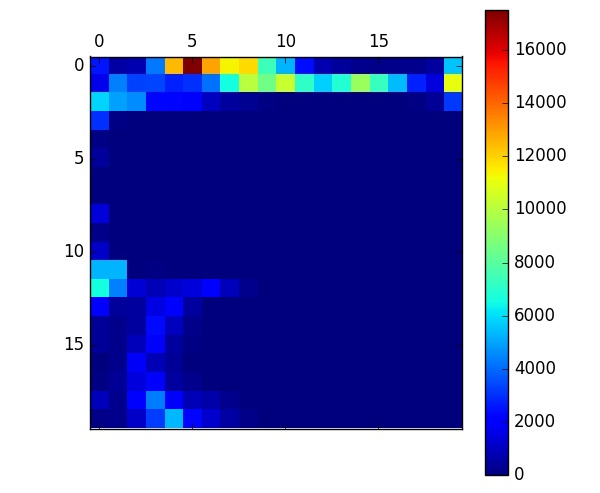
\includegraphics[scale=0.35]{../img/joint_histogram}
            \end{figure}
            
            \column{0.3\textwidth}
            \centering
            Mean:
            $$ \mu = \frac{1}{n} \sum_{i = 1}^{n} x_i $$
            Variance:
            $$ \operatorname {Var} (X)=\sum _{i=1}^{n}p_{i}\cdot (x_{i}-\mu )^{2} $$
        \end{columns}
    \end{myframe}
    
    \section{Classifiers}
    
    \subsection{Tree and random forest}
    
    \begin{myframe}
        \centering
        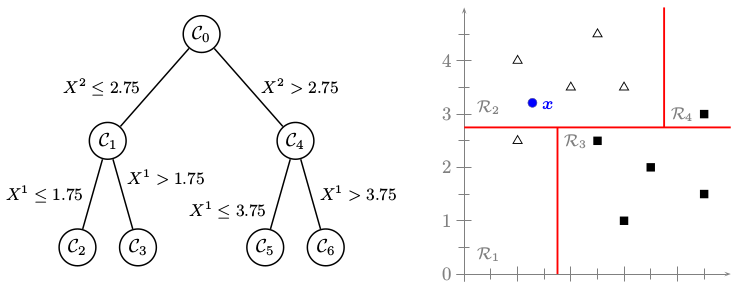
\includegraphics[scale=0.55]{../img/decision_tree_simple_example}
    \end{myframe}
    
    \subsection{SVM}
    
    \begin{myframe}
        \centering
        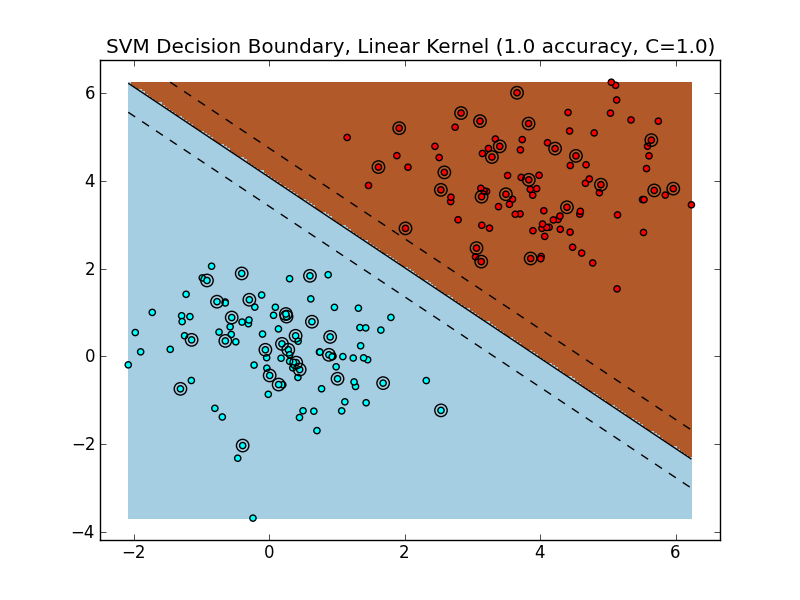
\includegraphics[scale=0.45]{../img/svm_linear}
    \end{myframe}
    
    \subsection{SVM and kernel trick}
    
    \begin{myframe}
        %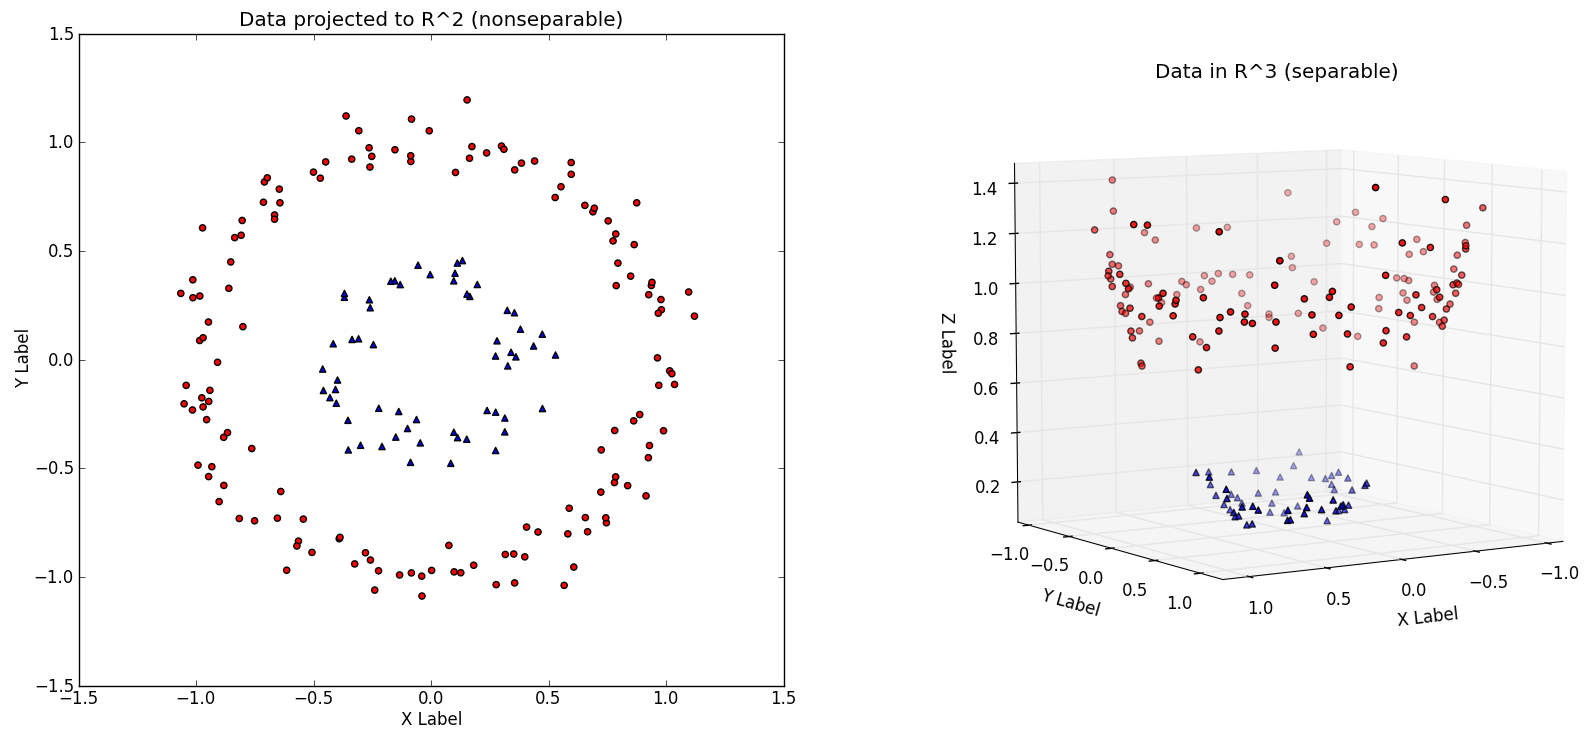
\includegraphics[scale=0.55]{../img/svm_data_2d_to_3d.png}
        \begin{center}
            \begin{tikzpicture}
                \node[anchor=south west,inner sep=0] (image) at (0,0) {
                    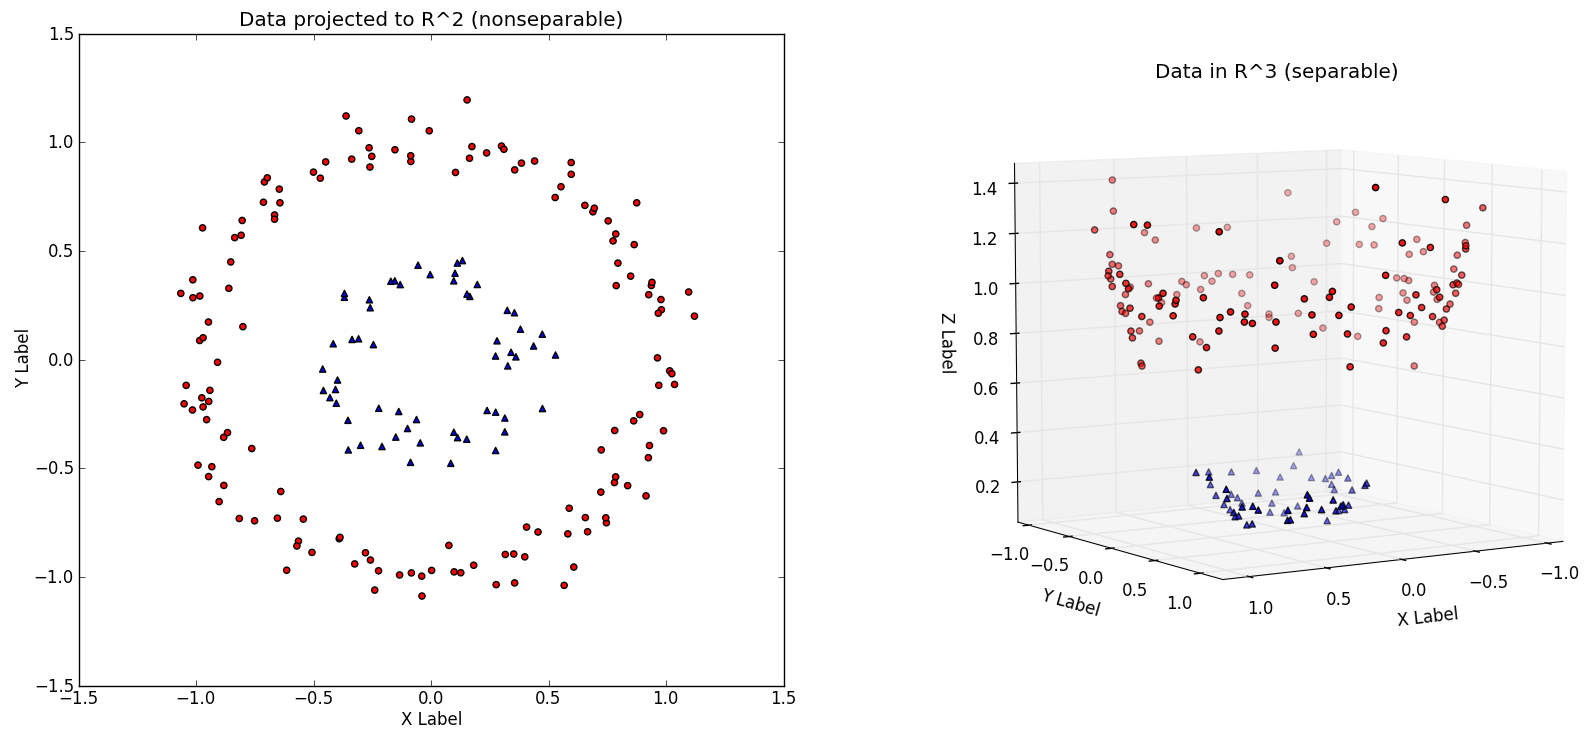
\includegraphics[scale=0.3]{../img/svm_data_2d_to_3d.png}
                };
                \onslide*<2->{
                    \node[align=center, color=black, fill=white, font={\Huge\bfseries}] at (image.center) {
                        $\chi^2$ kernel : 
                        $k(x,y) = 1 - \displaystyle\sum_{i=1}^n \frac{(x_i-y_i)^2}{\frac{1}{2}(x_i+y_i)}$
                    }
                };
            \end{tikzpicture}
        \end{center}
        
        
        %Example of kernel: kernel function: 
        
    \end{myframe}
    
    \subsection{CNN}
    
    \begin{myframe}
        Convolutional Neural Networks are very similar to ordinary Neural Networks from the previous chapter: they are made up of neurons that have learnable weights and biases. Each neuron receives some inputs, performs a dot product and optionally follows it with a non-linearity. The whole network still expresses a single differentiable score function: from the raw image pixels on one end to class scores at the other. And they still have a loss function (e.g. SVM/Softmax) on the last (fully-connected) layer and all the tips/tricks we developed for learning regular Neural Networks still apply.
        
        mainly use when the input is an image: neurons arranged in 3 dimensions: width, height, depth
        
        Main layer:
        Convolutional layer
        Pooling layer
        Activation layer: mainly relu (rectified linear unit): max(0, x)
        Fully-connected layer
    \end{myframe}
    
    \section{Segmentation}
    
    \begin{myframe}
        CNN pre-trained for saliency detection (PASCAL VOC / 19 layers)
    \end{myframe}
    
    \section{Results}
    
    \subsection{Segmentation}
    
    \begin{myframe}
        Precision, recall, accuracy (+ their definition)
        
        Result for UECFOOD 256
        
        (Display graph of the accuracy / recall / precision function of the overlaping value)
    \end{myframe}
    
    \subsection{Classification}
    
    \begin{myframe}
        Results for :
        - CNN as feature descriptors
        - Color histogram
        - BoW
        
        Compare to other results
    \end{myframe}
    
    \subsection{Segmentation followed by classification}
    
    \begin{myframe}
        Combining segmentation and classification:
        % 256:
        Overall accuracy: 28 \%
        74 \% for segmentation
        38 \% for classification
        
        % 100:
        Overall accuracy: 33 \%
        67 \% for segmentation
        50 \% for classification
        
        Compare to other results
        
        (Show the 5 best / least classes' accuracy)
        (Show the most confusing items)
    \end{myframe}
    
    \section{Future work}
    
    \begin{myframe}
        Regroup the classification in 5 big categories
    \end{myframe}
    
    \section{References}
    
    \begin{myframe}[t, allowframebreaks]
        \printbibliography[heading=none]
    \end{myframe}
    
    \section{Question}
    
    {
        % Disable footline for this frame
        \setbeamertemplate{footline}{} 
        \begin{frame}{Food log analysis - Baptiste NOGARET}{}
            \begin{columns}
                \column{0.5\textwidth}
                Segmentation and classfication applied on two reference datasets
                
                Obtain better segmentation than the reference
                
                Overall accuracy of 28 \% (to date, best result is 36 \% in ...).
                
                \column{0.5\textwidth}
                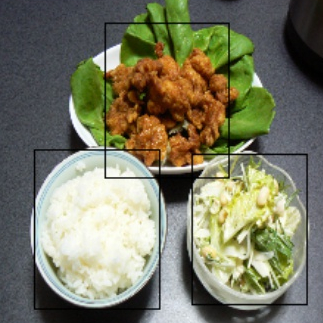
\includegraphics[width=\textwidth]{../img/seg_97_gt}
            \end{columns}
        \end{frame}
    }
   
\end{document}